\documentclass{exam}
\usepackage[utf8]{inputenc}
\usepackage{amsmath}
\usepackage{amssymb}
\usepackage{graphicx}
\usepackage{multicol}
\usepackage{pgfplots}
\usepackage{tkz-euclide}
\usetkzobj{all}

\newcommand{\class}{MAT -- 112}
\newcommand{\term}{Spring 2018}
\newcommand{\examnum}{Review 1 Solutions}
\newcommand{\examdate}{Dates: 2/5 -- 2/9}

\pagestyle{head}
\firstpageheader{}{}{}
\runningheader{\textbf{Start Time:}}{\textbf{End Time:}}{}
\runningheadrule

\begin{document}

\noindent
\begin{tabular*}{\textwidth}{l @{\extracolsep{\fill}} r @{\extracolsep{6pt}} l}
\textbf{\class} & \textbf{Name:} & \makebox[2in]{\hrulefill}\\
\textbf{\term} &&\\
\textbf{\examnum} &&\\
\textbf{\examdate} & \textbf{Pledge:}	& \makebox[2in]{\hrulefill}\\
\end{tabular*}\\
\rule[2ex]{\textwidth}{2pt}

\begin{center}
\fbox{\fbox{\parbox{5.5in}{\centering
Each question topic and the point value is recorded in the tables below. You may review these topics from any resource at your leisure. Once you decide to start a review problem, you are on the clock and you must work without any external resources, including no calculator. Each problem can be done one at a time but must be finished in a single sitting. Answer each question in the space provided, if you run out of space, then you may continue on the back of the page. It is your responsibility to plan out your time to ensure that you can finish all problems within the $2.0$ hours allotted. By writing your name and signing the pledge you are stating that your work adheres to these terms and the Davidson honor code. }}}
\end{center}

\vspace*{1em}

\begin{multicols}{2}
%% Scoring Table
\centering
\textbf{Scoring Table}\\
\addpoints
\gradetable[v][questions]

\columnbreak
%% Topics Table
\centering
\textbf{Topics Table}\\
\renewcommand{\arraystretch}{1.5}
\begin{tabular}{| c | c |}
\hline
Question & Topic\\
\hline
1 & Polynomial and Rational Functions\\
\hline
2 & Exponential and Log Functions\\
\hline
3 &  Trigonometric Functions\\
\hline
4 & Applications \\
\hline
&\\
\hline
\end{tabular}
\end{multicols}

\vspace*{2em}
%%Time Table
\begin{center}
\textbf{Time Table}\\
\renewcommand{\arraystretch}{2.5}
\begin{tabular}{| c | c | c | c | c | c | c | c | c | }
\hline
Question & ~~~~1~~~~ & ~~~~2~~~~ & ~~~~3~~~~ & ~~~~4~~~~ \\
\hline
Time & & & &  \\
\hline
\end{tabular}
\end{center}

\newpage

\begin{questions}

\question Let
\[
f(x)=2x^{2}-12x+19~\text{ and }~g(x)=\frac{3x-2}{2x+1}.
\]
\begin{parts}
\part[6]	On separate graphs, sketch a plot of the functions $f$ and $g$. 
Clearly label any $x$-intercepts, $y$-intercepts, and vertical and horizontal asymptotes.\\~\\
\textbf{Solution.}
\begin{figure}[h]
\centering
\begin{tikzpicture}
\begin{axis}[
	width=0.45\textwidth,
	axis lines = left,
	xlabel = $x$,
	ylabel = $f(x)$,
	xmin=0, xmax=6,
	ymin=0, ymax = 15,
]
\addplot [
	domain = 0:6,
	samples = 200,
	color = blue,
]
{2*x^2-12*x+19};
\end{axis}
\end{tikzpicture}
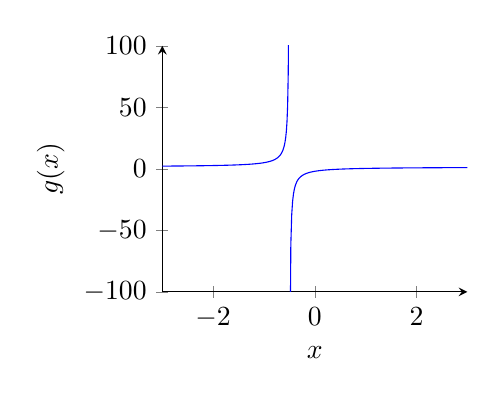
\begin{tikzpicture}
\begin{axis}[
	width=0.45\textwidth,
	axis lines = left,
	xlabel = $x$,
	ylabel = $g(x)$,
	xmin = -3, xmax = 3,
	ymin = -100, ymax = 100
]
\addplot [
	domain = -3:-0.51,
	samples = 200,
	color = blue,
]
{(3*x-2)/(2*x+1)};
\addplot [
	domain = -0.49:3,
	samples = 200,
	color = blue,
]
{(3*x-2)/(2*x+1)};
\end{axis}
\end{tikzpicture}
\end{figure}
The function $f(x)$ has no vertical or horizontal asymptotes, and no $x$-intercepts. It has a $y$-intercept at $(0,19)$. In order to plot $f$ accurately you will need to know its vertex: $(3,1)$. The function $g(x)$ has a vertical asymptote: $x=-1/2$, a horizontal asymptote: $y=3/2$, $x$-intercept at $(2/3,0)$ and $y$-intercept at $(0,-2)$. 
\part[4]	State the definition of the domain and range and find the domain and range of $f$ and $g$. \\~\\
\textbf{Solution.}	The domain of a function is the set of all possible values for the independent variable, and the range is the set of all corresponding output values. The domain of $f$ is $(-\infty,\infty)$ and the range of $f$ is $[1,\infty)$. The domain of $g$ is $(-\infty,-1/2)\cup(1/2,\infty)$ and the range of $g$ is $(-\infty,3/2)\cup(3/2,\infty)$. 
\end{parts}

\newpage

\question	
\begin{parts}
\part[5]	Solve each of the following equations for $x$. Leave your answer in exact fully simplified form.
\begin{itemize}
\item	$-11+5e^{x-3}=17$
\item	$\ln(x-2)+\ln(x-1)=2\ln(x+1)$
\item	$\log_{4}(x)-\log_{5}(x-1)=\frac{1}{2}$ (Note the different log bases, this is not a typo.)
\end{itemize}
\textbf{Solution.}
\begin{itemize}
\item	$-11+5e^{x-3}=17$ can be written as $e^{x-3}=28/5$. Taking the natural log of both sides gives us $x-3=\ln(28/5)$. Therefore,
\[
x=\ln(28/5)+3. 
\]
\item	$\ln(x-2)+\ln(x-1)=2\ln(x+1)$ can be written as $\ln(x-2)(x-1)=\ln(x+1)^{2}$. Taking the natural exponent of both sides we have $(x-2)(x-1)=(x+1)^{2}$. Expanding out gives us $x^{2}-3x+2=x^{2}+2x+1$. Therefore,
\[
x=1/5. 
\]
\item	$\log_{4}(x)-\log_{5}(x-1)=1/2$ can be written as $\log_{4}(x)-\frac{\log_{4}(x-1)}{\log_{4}(5)}=\log_{4}(2)$. By multiplying both sides by $\log_{4}(5)$ we can write this equation as $\log_{4}(5)\log_{4}(x)-\log_{4}(x-1)=\log_{4}(5)\log_{4}(2)$. Let $r=\log_{4}(5)$ and note that $r$ must be slightly greater than $1$. Then, we have
\[
\log_{4}(\frac{x^{r}}{x-1})=\log_{4}(2^{r}).
\]
Therefore, we see that $\frac{x^{r}}{x-1}=2^{r}$. In general this equation has two solutions, but finding both cannot be done by hand. However, one of the solutions is easy to identify, it is $x=2$. Verify for yourself that this satisfies the above equation. 
\end{itemize}
\part[5]	Use the definition of exponential and logarithmic functions to show that $f(x)=a^{x}$ and $g(x)=\log_{a}(x)$, where $a>0$ and $a\neq 1$, are inverse functions.\\~\\
\textbf{Solution.} We must show that $(f\circ g)(x)=(g\circ f)(x)=x$. To this end, note that $(f\circ g)(x)=a^{\log_{a}(x)}$ and $(g\circ f)(x)=\log_{a}(a^{x})$. Recall that $y=\log_{a}(x)$ if and only if $a^{y}=x$. It follows immediately that $(f\circ g)(x)=x$ and $(g\circ f)(x)=x$. 
\part[5]	Sketch a graph with a plot of $f(x)=2^{x}$ and $g(x)=\log_{2}(x)$. Be sure to label three points for both $f$ and $g$.\\~\\
\textbf{Solution.}
\begin{figure}[h]
\centering
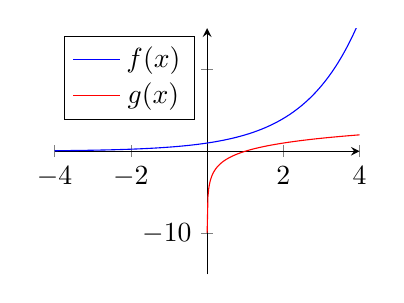
\begin{tikzpicture}
\begin{axis}[
	width=0.45\textwidth,
	axis lines = middle,
	xmin=-4, xmax=4,
	ymin=-15, ymax = 15,
	legend pos = north west,
]
\addplot [
	domain = -4:4,
	samples = 200,
	color = blue,
]
{pow(2,x)};
\addlegendentry{$f(x)$}
\addplot [
	domain = 0.001:4,
	samples = 200,
	color = red,
]
{log2(x)};
\addlegendentry{$g(x)$}
\end{axis}
\end{tikzpicture}
\end{figure}
Examples of three points you could choose are $(-1,1/2),~(0,1),~(1,2)$ for $f(x)$ and $(1/2,-1),~(1,0),~(2,1)$ for $g(x)$. 
\end{parts}

\newpage

\question
\begin{parts}
\part[5]	State the definition of the trigonometric functions: cosine, sine, and tangent; include a clearly labeled diagram.\\~\\
\textbf{Solution.}	Consider the point $(x,y)$ that forms the right triangle drawn below.
\begin{figure}[h]
\centering
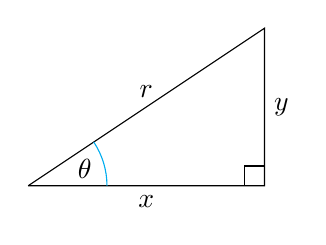
\begin{tikzpicture}
	\coordinate (C) at (-1.5cm,-1.0cm);
	\coordinate (A) at (1.5cm,-1.0cm);
	\coordinate (B) at (1.5cm,1.0cm);
 	\draw (C) -- node[above] {$r$} (B) -- node[right] {$y$} (A) -- node[below] {$x$} (C);
  	\draw (1.25cm,-1.0cm) rectangle (1.5cm,-0.75cm);
  	\tkzMarkAngle[size=1cm,color=cyan](A,C,B);
	\tkzLabelAngle[pos = 0.75](A,C,B){$\theta$}
\end{tikzpicture}
\end{figure}~\\
Note that $r=\sqrt{x^{2}+y^{2}}$ and we have the following definitions
\[
\cos\theta=\frac{x}{r},~\quad\sin\theta=\frac{y}{r},~\quad\tan\theta=\frac{y}{x}.
\]
\part[5]	Draw the 30-60-90 and 45-45-90 right triangles and state the cosine, sine, and tangent of the 30, 45, and 60 degree angles. \\~\\
\textbf{Solution.}
\begin{figure}[h]
\centering
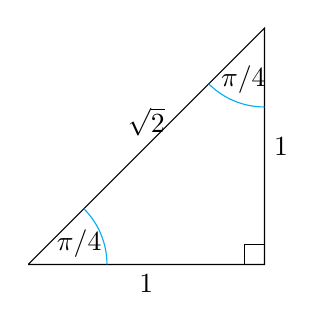
\begin{tikzpicture}
	\coordinate (C) at (-1.5cm,-1.5cm);
	\coordinate (A) at (1.5cm,-1.5cm);
	\coordinate (B) at (1.5cm,1.5cm);
 	\draw (C) -- node[above] {$\sqrt{2}$} (B) -- node[right] {$1$} (A) -- node[below] {$1$} (C);
  	\draw (1.25cm,-1.5cm) rectangle (1.5cm,-1.25cm);
  	\tkzMarkAngle[size=1cm,color=cyan](A,C,B);
	\tkzLabelAngle[pos = 0.70](A,C,B){$\pi/4$}
	\tkzMarkAngle[size=1cm,color=cyan](C,B,A);
	\tkzLabelAngle[pos = 0.70](C,B,A){$\pi/4$}
\end{tikzpicture}
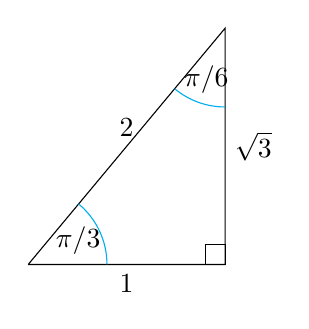
\begin{tikzpicture}
	\coordinate (C) at (-1.5cm,-1.5cm);
	\coordinate (A) at (1.0cm,-1.5cm);
	\coordinate (B) at (1.0cm,1.5cm);
 	\draw (C) -- node[above] {$2$} (B) -- node[right] {$\sqrt{3}$} (A) -- node[below] {$1$} (C);
  	\draw (1.0cm,-1.5cm) rectangle (0.75cm,-1.25cm);
  	\tkzMarkAngle[size=1cm,color=cyan](A,C,B);
	\tkzLabelAngle[pos = 0.70](A,C,B){$\pi/3$}
	\tkzMarkAngle[size=1cm,color=cyan](C,B,A);
	\tkzLabelAngle[pos = 0.70](C,B,A){$\pi/6$}
\end{tikzpicture}
\end{figure}~\\
From the above figures it is easy to find the cosine, sine, and tangent of these special angles.
\begin{align*}
\cos(\pi/6)=\frac{\sqrt{3}}{2}\quad\sin(\pi/6)=\frac{1}{2}\quad\tan(\pi/6)=\frac{1}{\sqrt{3}} \\
\cos(\pi/4)=\frac{1}{\sqrt{2}}\quad\sin(\pi/4)=\frac{1}{\sqrt{2}}\quad\tan(\pi/4)=1 \\
\cos(\pi/3)=\frac{1}{2}\quad\sin(\pi/3)=\frac{\sqrt{3}}{2}\quad\tan(\pi/3)=\sqrt{3}
\end{align*}
\part[5]	Sketch a graph with the plot of the cosine, sine, and tangent functions on the interval $[-\pi,\pi]$. \\~\\
\textbf{Solution.}
\begin{figure}[h]
\centering
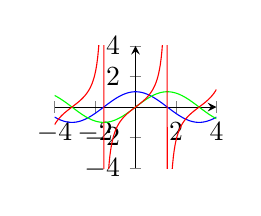
\begin{tikzpicture}
\begin{axis}[
	width=0.30\textwidth,
	axis lines = middle,
	xmin=-4, xmax=4,
	ymin=-4, ymax = 4,
	legend pos = north west,
]
\addplot [
	domain = -4:4,
	samples = 200,
	color = blue,
]
{cos(deg(x))};
\addplot [
	domain = -4:4,
	samples = 200,
	color = green,
]
{sin(deg(x))};
\addplot [
	domain = -4:4,
	samples = 200,
	color = red,
]
{tan(deg(x))};
\end{axis}
\end{tikzpicture}
\end{figure}
\end{parts}

\newpage

\question
\begin{parts}
\part[5]	A simple pendulum, see figure below, 
\begin{figure}[h]
\centering
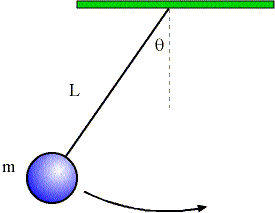
\includegraphics[scale=0.5]{review1_fig1}
\end{figure}
consists of a mass $m$ hanging from a string of length $L$ from a fixed pivot point. When displaced to an initial angle $\theta_{0}$ and released, the pendulum will swing back and forth with periodic motion described by the equation
\[
\theta(t)=\theta_{0}\cos(\sqrt{\frac{g}{L}} t),
\]
where $g$ is the force of gravity and $t$ is the time elapsed since the mass was released.
\begin{itemize}
\item	Express the period of the pendulum's motion in terms of the variables described above. 
\item	When is the displacement maximized and when is it zero?
\end{itemize}
\textbf{Solution.}	The period of the pendulum is given by $\frac{2\pi}{\sqrt{g/L}}$. Furthermore, the pendulum has maximum displacement when $\sqrt{\frac{g}{L}}t=0,\pi,\ldots$, i.e. when $t=0,\pi\sqrt{\frac{L}{g}},\ldots,$; the pendulum has zero displacement when $\sqrt{\frac{g}{L}}t=\pi/2,3\pi/2,\ldots$, i.e. when $t=(\pi/2)\sqrt{\frac{L}{g}},(3\pi/2)\sqrt{\frac{L}{g}},\ldots$. 
\part[5]	The half life of Carbon-14 is 5730 years. The amount left of an initial sample $y_{0}$ (measured in grams) can be modeled by
\[
y(t)=y_{0}e^{rt}.
\]
\begin{itemize}
\item	Find the decay rate $r$. Leave your answer in exact fully simplified form. 
\item	If $2$ grams remain after $1000$ years, find the initial sample $y_{0}$. Leave your answer in exact fully simplified form. 
\end{itemize}
\textbf{Solution.}	The decay rate can be found by noting that $\frac{1}{2}=e^{r(5730)}$. Taking the natural log of both sides gives $r=\frac{\ln(1/2)}{5730}$. If $2$ grams remain after $1000$ years, then we have $2=y_{0}e^{r(1000)}$, which we can use to solve for $y_{0}$ as follows.
\begin{align*}
y_{0}&=\frac{2}{e^{r(1000)}} \\
&=\frac{2}{e^{\ln(1/2)/5.73}} \\
&=\frac{2}{e^{\ln(1/2)^{1/5.73}}} \\
&=\frac{2}{(1/2)^{1/5.73}}.
\end{align*}
\end{parts}
\end{questions}


\end{document}